\documentclass[border=10pt]{standalone}
\usepackage[svgnames]{xcolor}
\usepackage{amsmath}
\usepackage{pgfplots}
\pgfplotsset{compat=newest}
\usepackage[sfdefault]{FiraSans}
\usepackage{FiraMono}
\renewcommand*\familydefault{\sfdefault}
\begin{document}
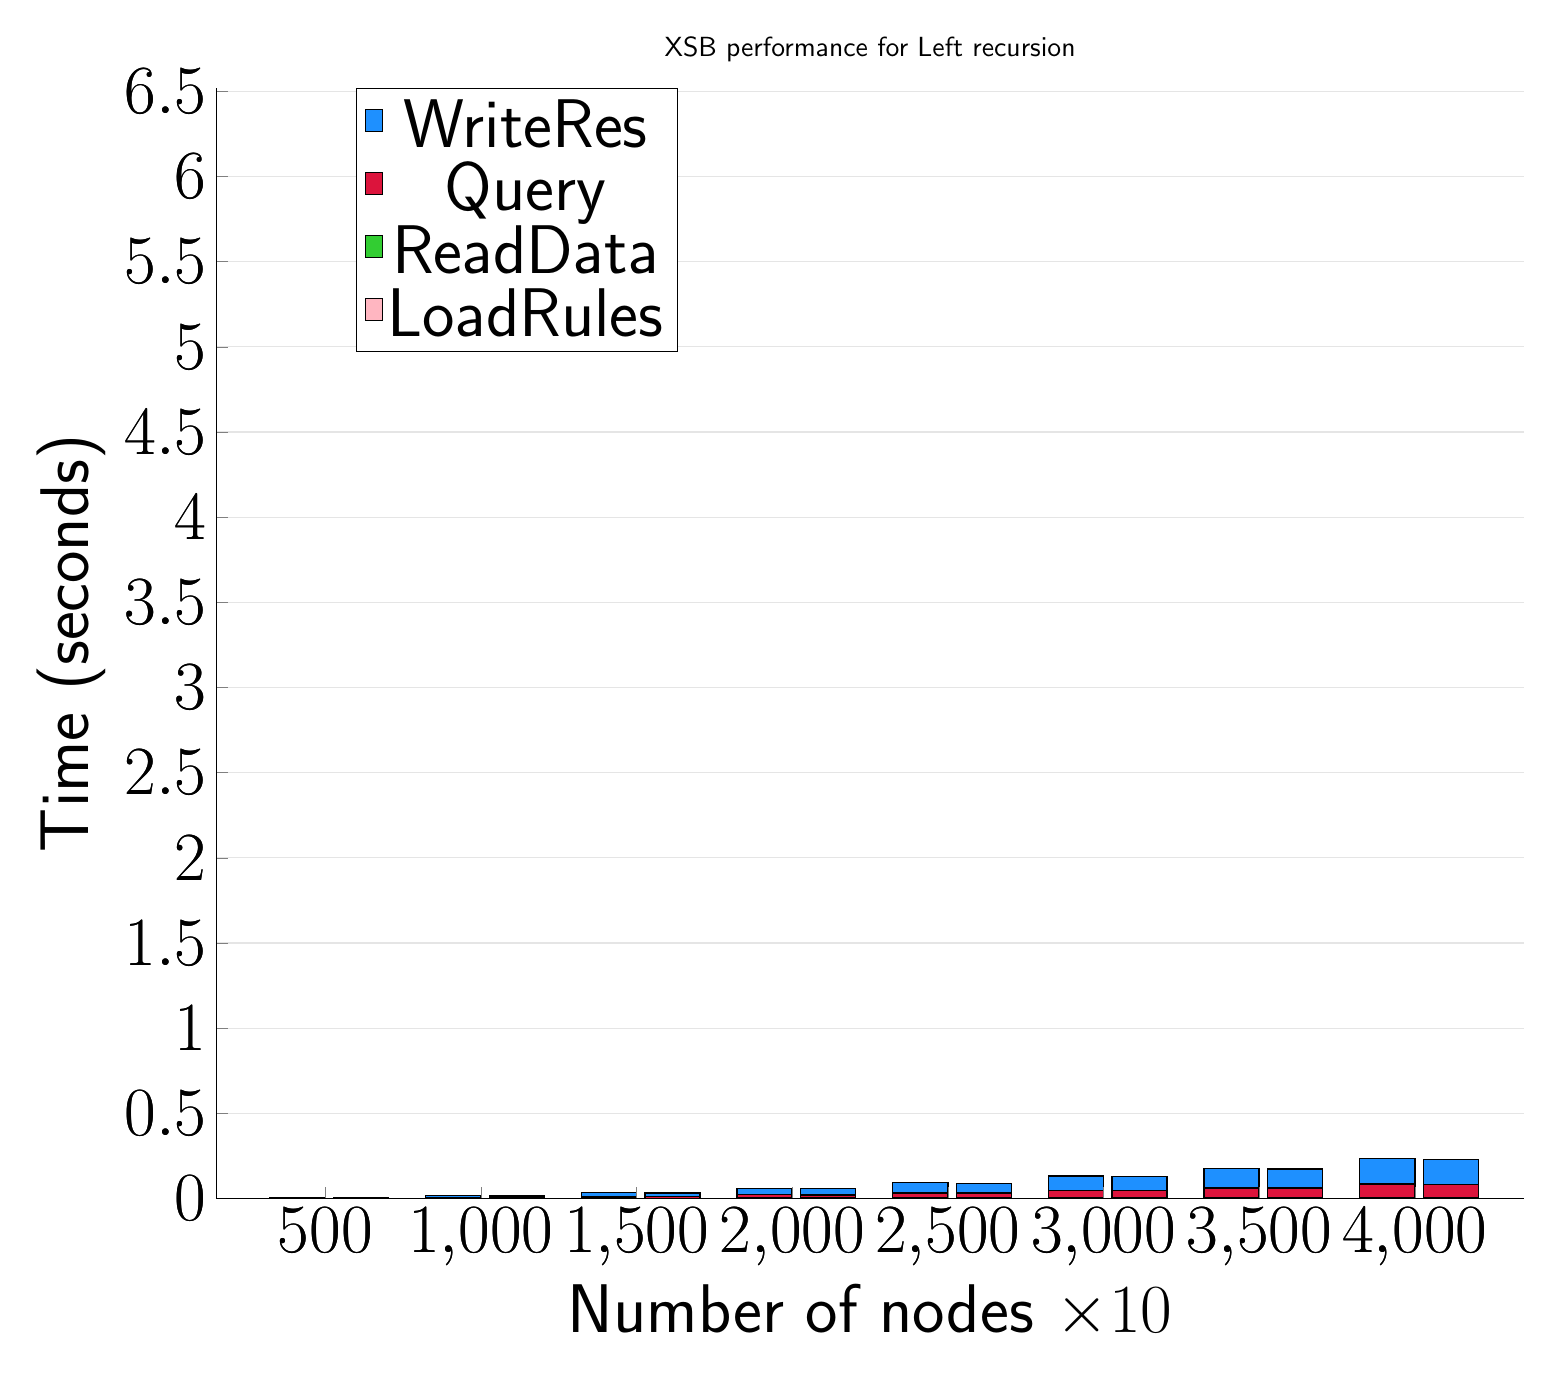
\begin{tikzpicture}
	\begin{axis}[
			ybar stacked,
			title={XSB performance for Left recursion},
			bar shift=-10pt,
			width=1.5\textwidth,
			bar width=0.7cm,
			ymajorgrids, tick align=inside,
			major grid style={draw=gray!20},
			xtick=data,
			ymin=0, ymax=6.52002317905426,
			axis x line*=bottom,
			axis y line*=left,
			enlarge x limits=0.1,
			legend style={
					at={(0.23, 1)},
					anchor=north,
					legend columns=1,
					font=\Huge,
				},
			ylabel={Time (seconds)},
			xlabel={Number of nodes $\times 10$},
			label style={font=\Huge},
			tick label style={font=\Huge},
		]
		\addlegendimage{fill=DodgerBlue, draw=black, line width=0.2pt}
		\addlegendentry{WriteRes}
		\addlegendimage{fill=Crimson, draw=black, line width=0.2pt}
		\addlegendentry{Query}
		\addlegendimage{fill=LimeGreen, draw=black, line width=0.2pt}
		\addlegendentry{ReadData}
		\addlegendimage{fill=LightPink, draw=black, line width=0.2pt}
		\addlegendentry{LoadRules}
		\addplot +[fill=LightPink, draw=black, line width=0.5pt] coordinates {
				(500, 0.00108184814453125)
				(1000, 0.0010629177093505848)
				(1500, 0.001038718223571777)
				(2000, 0.0010597467422485349)
				(2500, 0.001108860969543457)
				(3000, 0.0012215614318847653)
				(3500, 0.00105750560760498)
				(4000, 0.0010768651962280269)
			};
		\addplot +[fill=LimeGreen, draw=black, line width=0.5pt] coordinates {
				(500, 0.0008192300796508789)
				(1000, 0.001359748840332033)
				(1500, 0.001873779296874998)
				(2000, 0.002380847930908202)
				(2500, 0.0029600381851196287)
				(3000, 0.0035553932189941414)
				(3500, 0.003986692428588866)
				(4000, 0.004564619064331055)
			};
		\addplot +[fill=Crimson, draw=black, line width=0.5pt] coordinates {
				(500, 0.001126813888549804)
				(1000, 0.004656839370727538)
				(1500, 0.010808229446411131)
				(2000, 0.01920464038848877)
				(2500, 0.029608368873596212)
				(3000, 0.04392406940460205)
				(3500, 0.057813191413879396)
				(4000, 0.07937197685241698)
			};
		\addplot +[fill=DodgerBlue, draw=black, line width=0.5pt] coordinates {
				(500, 0.002525877952575684)
				(1000, 0.009744215011596672)
				(1500, 0.021582674980163575)
				(2000, 0.03801326751708982)
				(2500, 0.059305429458618164)
				(3000, 0.08433966636657715)
				(3500, 0.11433496475219732)
				(4000, 0.1489773750305176)
			};
	\end{axis}
	\begin{axis}[
			ybar stacked,
			bar shift=13pt,
			width=1.5\textwidth,
			bar width=0.7cm,
			ymajorgrids, tick align=inside,
			major grid style={draw=none},
			xtick=data,
			ymin=0, ymax=6.52002317905426,
			axis x line*=none,
			axis y line*=none,
			enlarge x limits=0.1,
			label style={font=\Huge},
			tick label style={font=\Huge},
		]
		\addplot +[fill=LightPink, draw=black, line width=0.5pt] coordinates {
				(500, 0.0006163999999999998)
				(1000, 0.0006118)
				(1500, 0.0006055000000000004)
				(2000, 0.0006146000000000004)
				(2500, 0.0006238000000000001)
				(3000, 0.0006349999999999996)
				(3500, 0.0006086999999999993)
				(4000, 0.0006159999999999997)
			};
		\addplot +[fill=LimeGreen, draw=black, line width=0.5pt] coordinates {
				(500, 0.0005880000000000002)
				(1000, 0.0010717)
				(1500, 0.0015432)
				(2000, 0.002051)
				(2500, 0.0025302000000000002)
				(3000, 0.0030497)
				(3500, 0.0034939999999999997)
				(4000, 0.0040036)
			};
		\addplot +[fill=Crimson, draw=black, line width=0.5pt] coordinates {
				(500, 0.0011064)
				(1000, 0.0045603)
				(1500, 0.010622900000000001)
				(2000, 0.0188502)
				(2500, 0.0291761)
				(3000, 0.0431721)
				(3500, 0.057005099999999996)
				(4000, 0.0783614)
			};
		\addplot +[fill=DodgerBlue, draw=black, line width=0.5pt] coordinates {
				(500, 0.0022721000000000004)
				(1000, 0.0093611)
				(1500, 0.0209868)
				(2000, 0.0367775)
				(2500, 0.0568887)
				(3000, 0.0822341)
				(3500, 0.11212)
				(4000, 0.14634699999999998)
			};
	\end{axis}
\end{tikzpicture}

\end{document}
